
\documentclass[template=tabling,81pt,headonall]{azmoon}
\usepackage{xepersian}
\usepackage{amsfonts}
\usepackage{graphicx}
\usepackage{svg}
\svgpath{ {./images/} }
\graphicspath{ {./images/} }
\settextfont{Yas}
\setdigitfont{A Iranian Sans}
\usepackage{fontawesome5}

\printanswers
    \teacher{محمد صالح علی اکبری}
    \teachertitle{دبیر}
    \city{گناباد}
    \schooltitle{متوسطه دوره اول}
    \school{مقداد}
    \grade{نهم}
    \branch{۱}
    \topic{ریاضی}
    \examdate{دی ۱۴۰۲}
    \answertime{۹۰ دقیقه}
    \begin{document}
	\begin{questions}
		\nointerlineskip%
		\vskip-\baselineskip
		\question[1]{%
هر یک از مجموعه‌های زیر چند عضو دارند؟
    \begin{parts}[1]\part{\{۴ ، ۶، ۸\}}
\part{\{۴ ، ۵، ۸\}}
\end{parts}

    }\question[2]{%
مجموعه $S=\{1,2,3,4,5,6,7,8\}$ به این صورت است. برای هر یک از زیر مجموعه‌های این مجموعه که در زیر آمده مانند نمونه یک جمله نظیر کنید.
    \begin{parts}[2]\part{$A=\{8 , 7\}$ مجموعه تمام اعداد عضو S که در تاس وجود ندارند.}
\part{$B=\{2 , 3 , 5 , 7 \}$}
\part{$C=\{6, 3\}$}
\end{parts}

    }\question[1]{%
حاصل عبارت‌های زیر را حساب کنید.
    \begin{LTR}
        \begin{parts}[2]\part{$ 42 - 60 + 100 = $}
\part{$20 - 70 + 10 =$}
\end{parts}
\end{LTR}
        
    }\question[1]{%
حاصل عبارت‌های زیر را حساب کنید.
    \begin{LTR}
        \begin{parts}[2]\part{$-5 \times (-3) = $}
\part{$-7 \times (3) = $}
\part{$3 \times (8)  = $}
\part{$3 \times (-4) = $}
\end{parts}
\end{LTR}
        
    }\question[2]{%
حاصل تقسیم‌های زیر را محاسبه کنید.
    \begin{parts}[4]\part{ 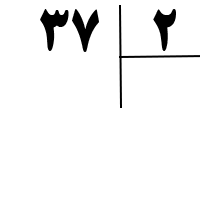
\includegraphics[scale = 0.18]{تقسیم2}}
\part{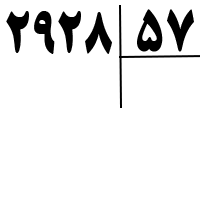
\includegraphics[scale = 0.18]{تقسیم10}}
\end{parts}
‌
\\‌
\\‌
\\
    }\question[3]{%
حاصل جمع و تفریق‌های زیر را محاسبه کنید.
    \begin{LTR}
        \begin{parts}[1]\part{$\dfrac{4}{3}-(-\dfrac{4}{8}) = $}
\part{$\dfrac{1}{2}-\dfrac{3}{1} = $}
\part{$-\dfrac{8}{4}+\dfrac{2}{1} = $}
\end{parts}
\end{LTR}
        
    }\question[2]{%
حاصل ضرب و تقسیم‌های زیر را محاسبه کنید.
    \begin{LTR}
        \begin{parts}[1]\part{$+\dfrac{4}{3}\times \dfrac{1}{8} = $}
\part{$\dfrac{1}{2}\div\dfrac{3}{2} = $}
\end{parts}
\end{LTR}
        
    }\question[4]{%
حاصل عبارت‌های زیر را حساب کنید. \\ $\sqrt{2} \simeq 1.2 \sqrt{3} \simeq 1.7 \sqrt{5} \simeq 2.2  \sqrt{6} \simeq 2.4 \sqrt{7} \simeq 2.6 \sqrt{8} \simeq 2.8$
    \begin{LTR}
        \begin{parts}[1]\part{$|\sqrt{2}-4| = $}
\part{$|\sqrt{12}-3| = $}
\part{$|\sqrt{7}-5| = $}
\part{$|\sqrt{4}-2| = $}
\end{parts}
\end{LTR}
        
    }\question[2]{%
اگر امروز ۲۳ دی باشد و اسفندماه ۲۹ روزه باشد. تا عید (اول فروردین) چند روز باقی مانده است؟}\question[2]{%
محیط و مساحت شکل زیر را محاسبه کنید. \\ 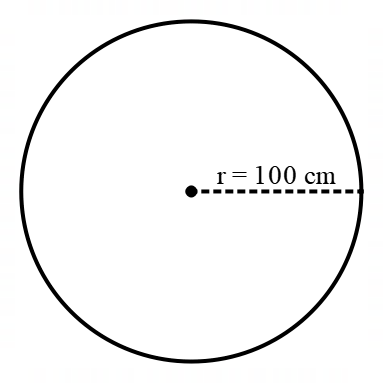
\includegraphics[scale = 1]{دایره}}\end{questions}
    \end{document}
    